If you haven't done so already, visit \url{https://www.libreoffice.org/download/download-libreoffice/} and download the Libr\'{e} Office suite.

Suppose a businessman was in the completely legitimate business of making loans to people who are regarded as poor credit risks by conventional banks.  Of course, he'd want to keep track of the loan amounts and the recipients.  A spreadsheet is the perfect tool!

Here's a screen shot of how the data might be recorded:

\centerline{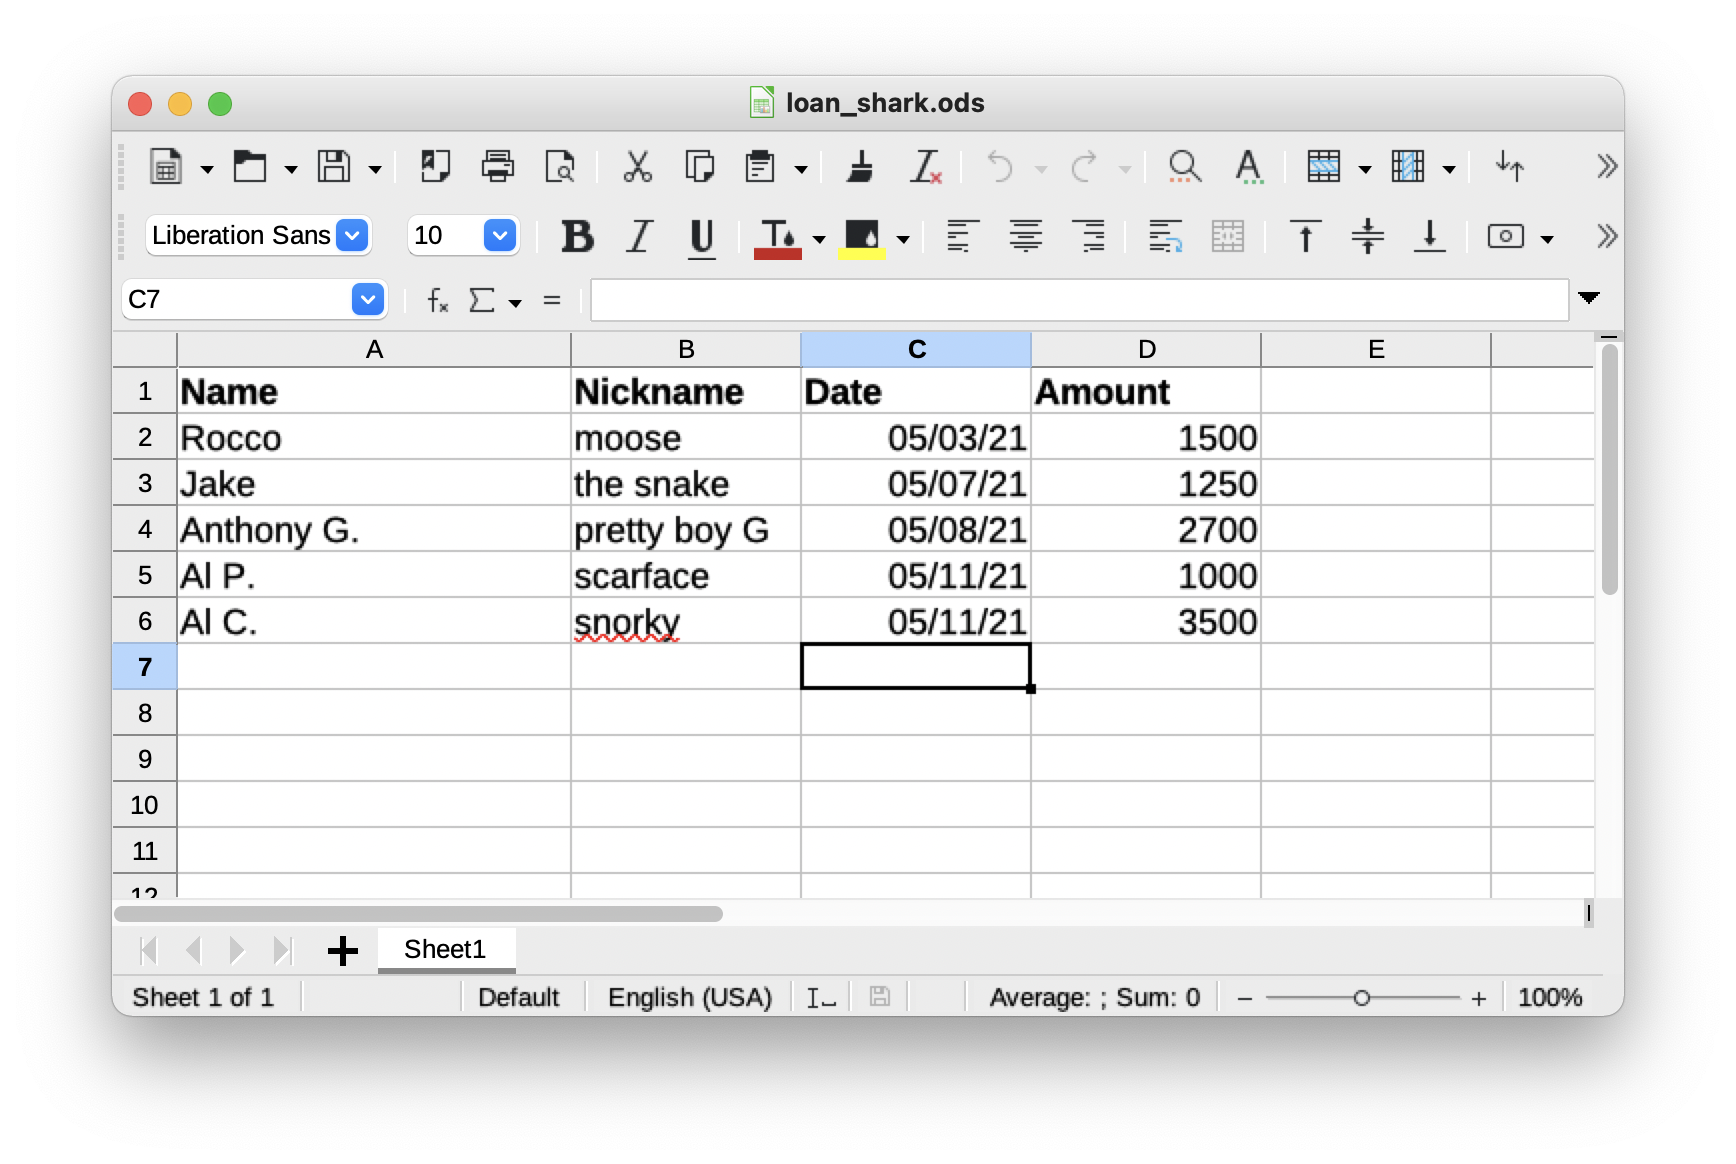
\includegraphics[scale=.5]{loans.png}}

We're using the free/open-source Libr\'{e} Office spreadsheet in the above.  There are other choices (Excel on Windows and Numbers on Apple computers) but all of them work in a similar way and Libr\'{e} Office is free.  Spreadsheet files created by Libr\'{e} Office have a .ods suffix.  

The stuff that you enter into a cell in a spreadsheet fall into two main categories: a cell can contain data, or a cell can contain a calculated value.  To make a ``calculation''-type cell you have to put an equals sign up front.  When you're doing a calculation you can use the values that are in other cells by referring to them by column (letter) followed by row (number).  For example the \$3500 that Snorky borrowed is in cell D6.

Some calculated cells are pretty simple, like the sum, difference or product of the values in other cells.
Other calculated cells can be pretty complex -- there are a lot of built-in functions that can be used to do these more difficult computations.  Once you know your way around, you'll probably just type the name of the function you need.  Until then there is the so-called ``function wizard.''  Try looking for a function that will give you random numbers.

\centerline{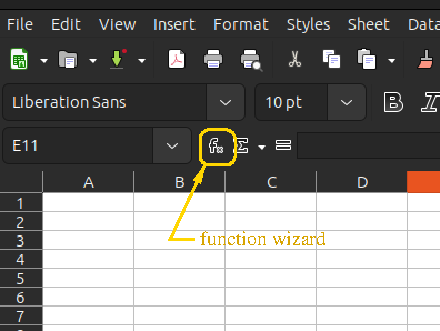
\includegraphics[scale=.5]{func_wiz.png}}

\subsubsection{tasks}

\begin{enumerate}

\item Open the loan shark spreadsheet (the file is available on the book website) and make some additions -- columns for monthly interest rate, due date and the current amount due.  You should verify that subtracting the values in two cells that are formatted as dates does the right thing.  Since you'll want time to be measured in months, what conversion needs to be applied?

\item Create a spreadsheet for keeping track of student grades in a math class. Use your favorite actors, sports stars, musicians (or whatever) as students, and just generate random numbers to put in as their grades. Make the homework grades (let's say 5 different scores) be on a scale from 0 to 10.  Make the quiz grades (also 5 of them) be on a scale from 0 to 20. Finally, make up two exam scores on a 0 to 100 scale.
Create subtotals for homework, quizzes and exams, also a grand total with homework weighted $20\%$, quizzes weighted
$30\%$ and exams weighted $50\%$.  

Many teachers have policies where the lowest grade in some category is dropped.  Figure out how to drop the lowest quiz score.

\end{enumerate}

